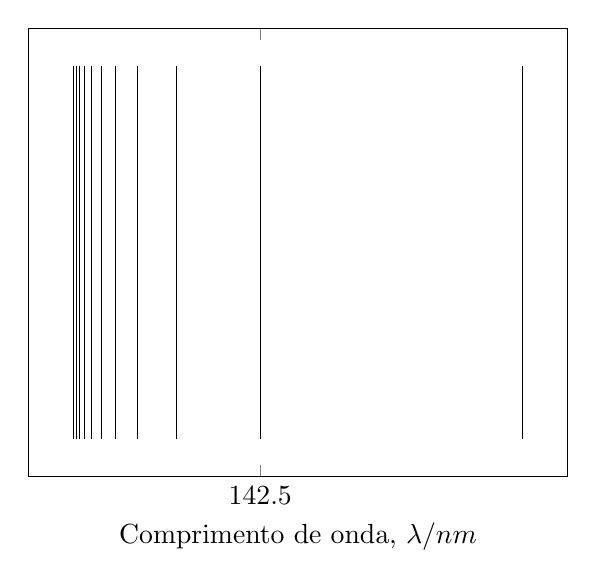
\begin{tikzpicture}
    \def\R{1000*8.314}% boltzmann constant
    \begin{axis}
        [
            domain = 0:2700,
            xlabel = {Comprimento de onda, $\lambda/\si{nm}$},
            xtick = {142.5}, 
            ytick=\empty,
        ]
    \pgfplotsinvokeforeach{4,5,6,7,8,9,10,11,12,13,14}
        {
            \addplot[black] coordinates
            {
                ((1240/13.6)/(1-9/#1^2), 0)
                ((1240/13.6)/(1-9/#1^2), 1)
            };
        }
\end{axis}
\end{tikzpicture}